\section{Results}

\subsection*{Public Dataset: COLO}

The organize dataset is published on the huggingface dataset repository. It's organized in two formats: YOLO and COCO

\subsection*{Evaluation Metrics}


\begin{figure}[h]
    \centering
    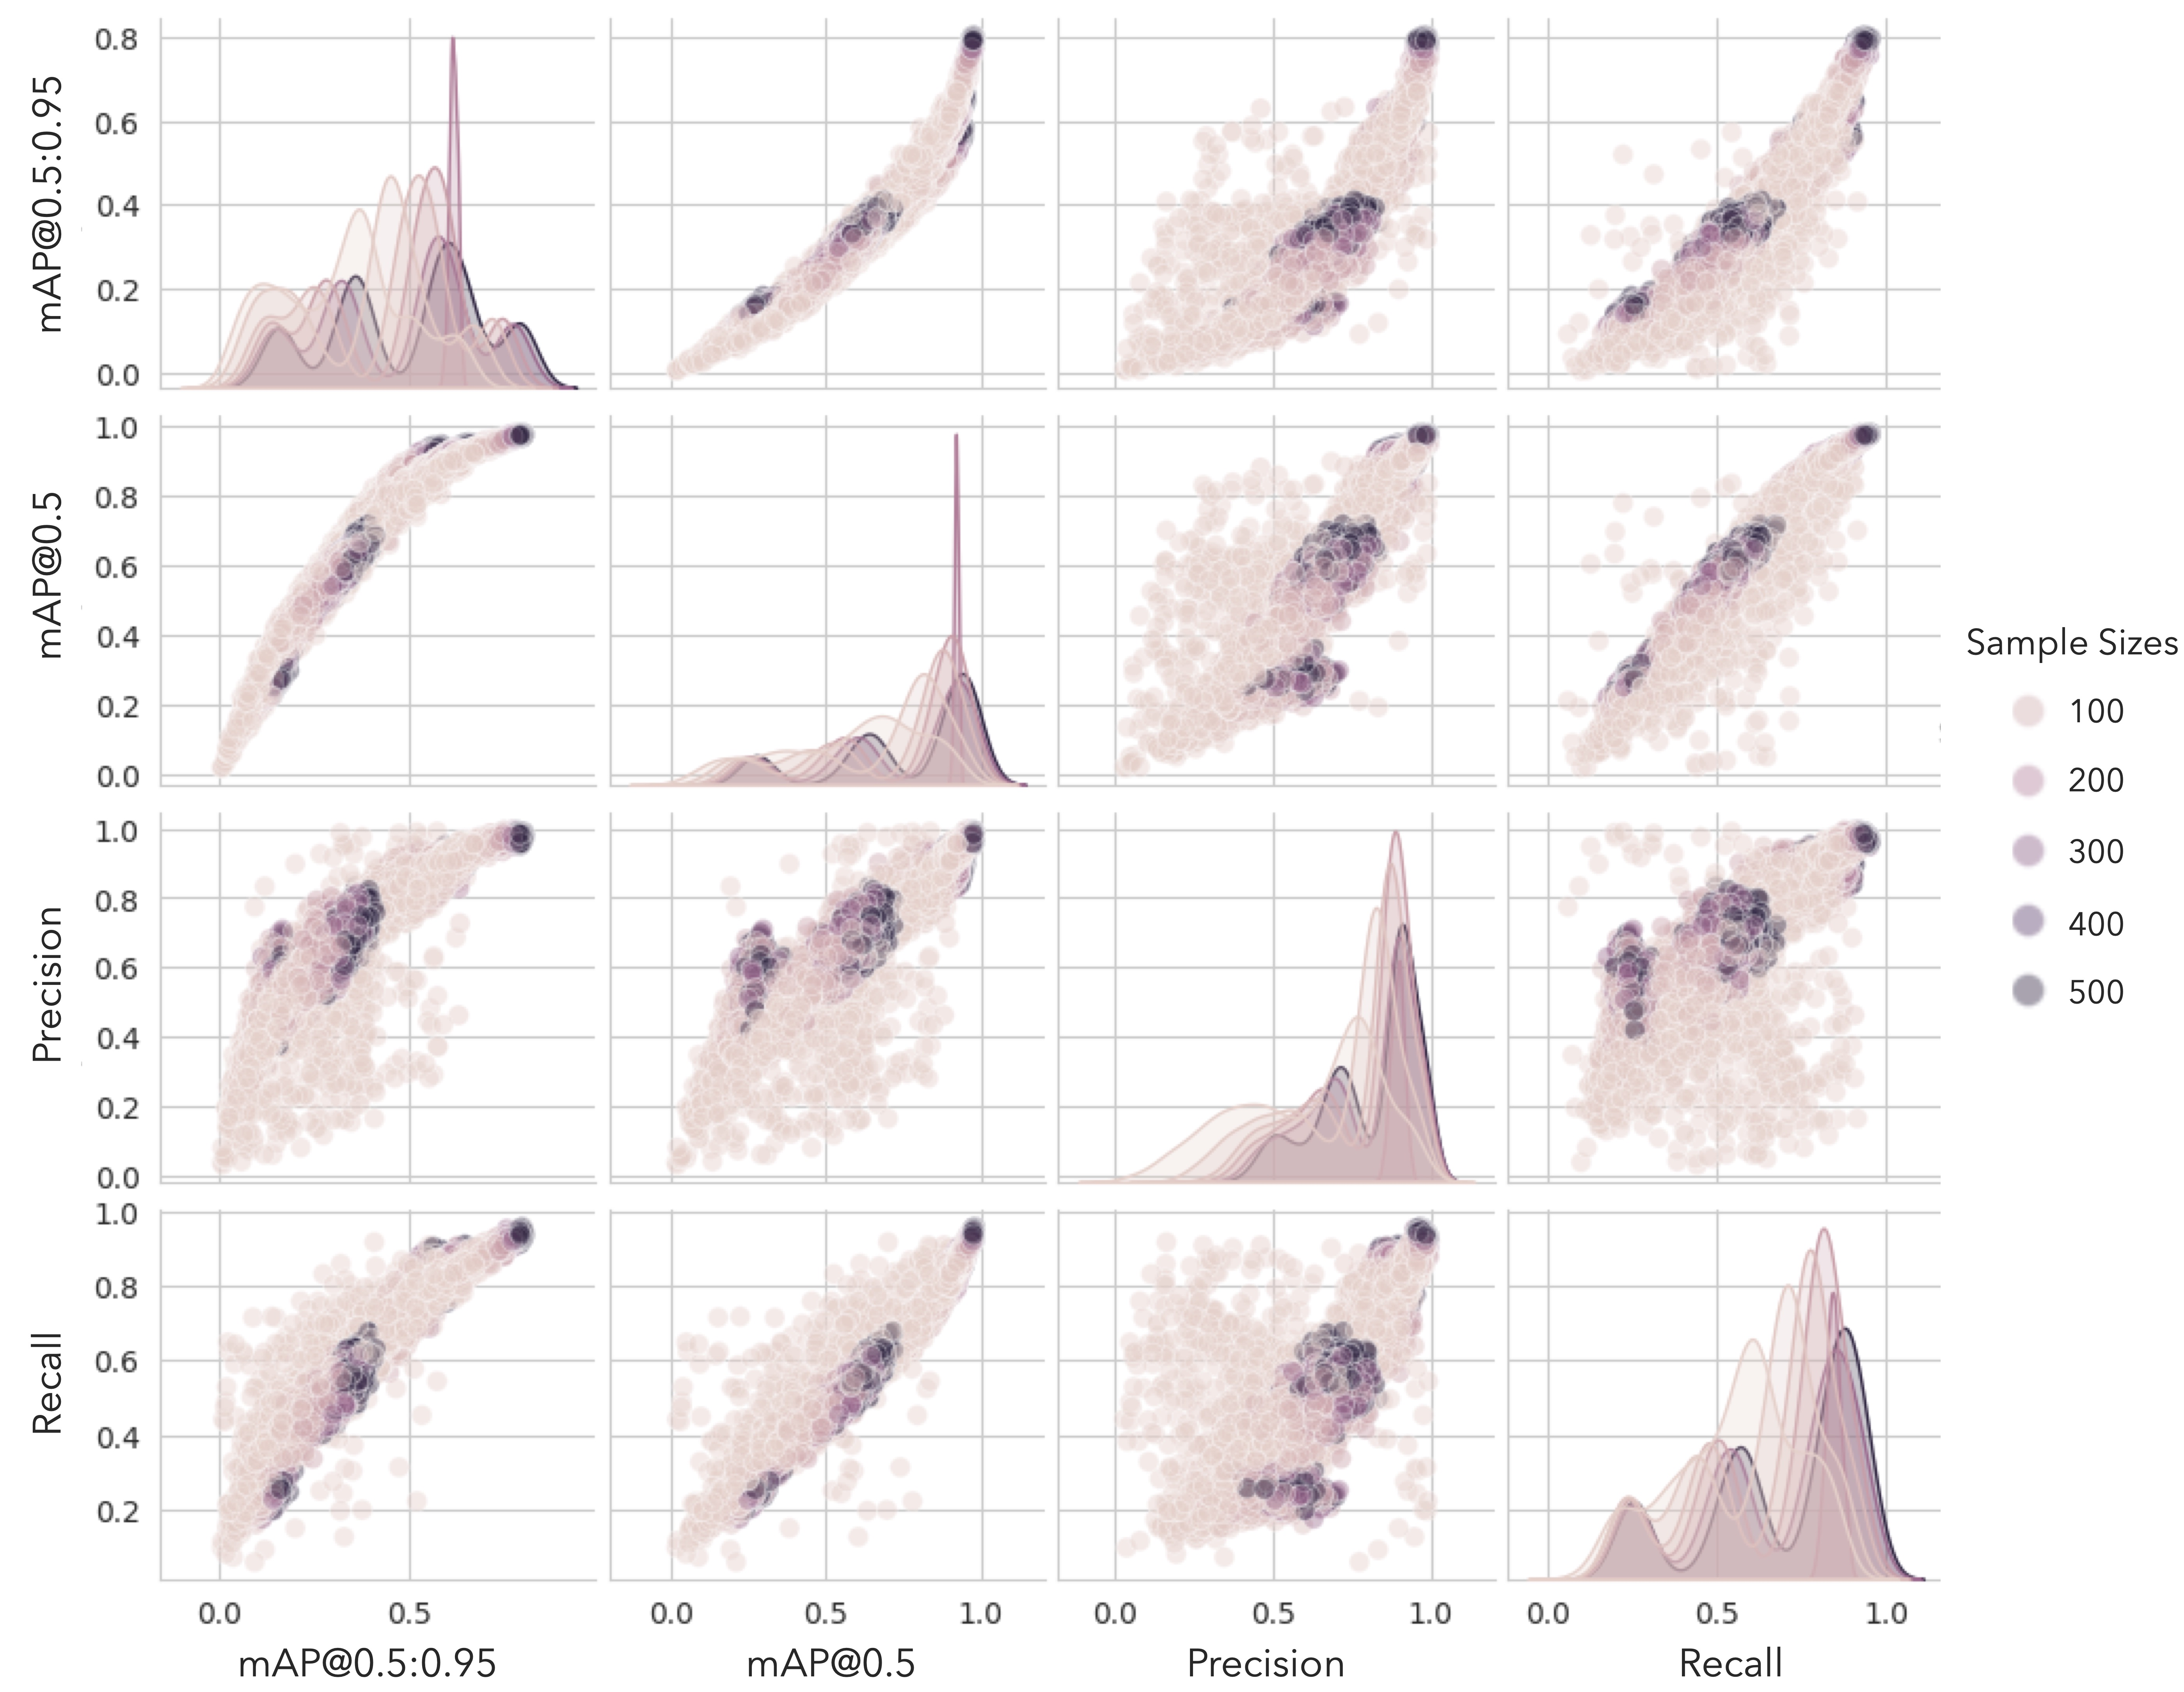
\includegraphics[width=1\textwidth]{figure_s1.jpg}
    \caption{Examples of the annotated images.}
    \label{fig:metrics}
\end{figure}



\subsection*{Study 1: The changes in camera view angles dramatically affect the model performance}


\begin{figure}[h]
    \centering
    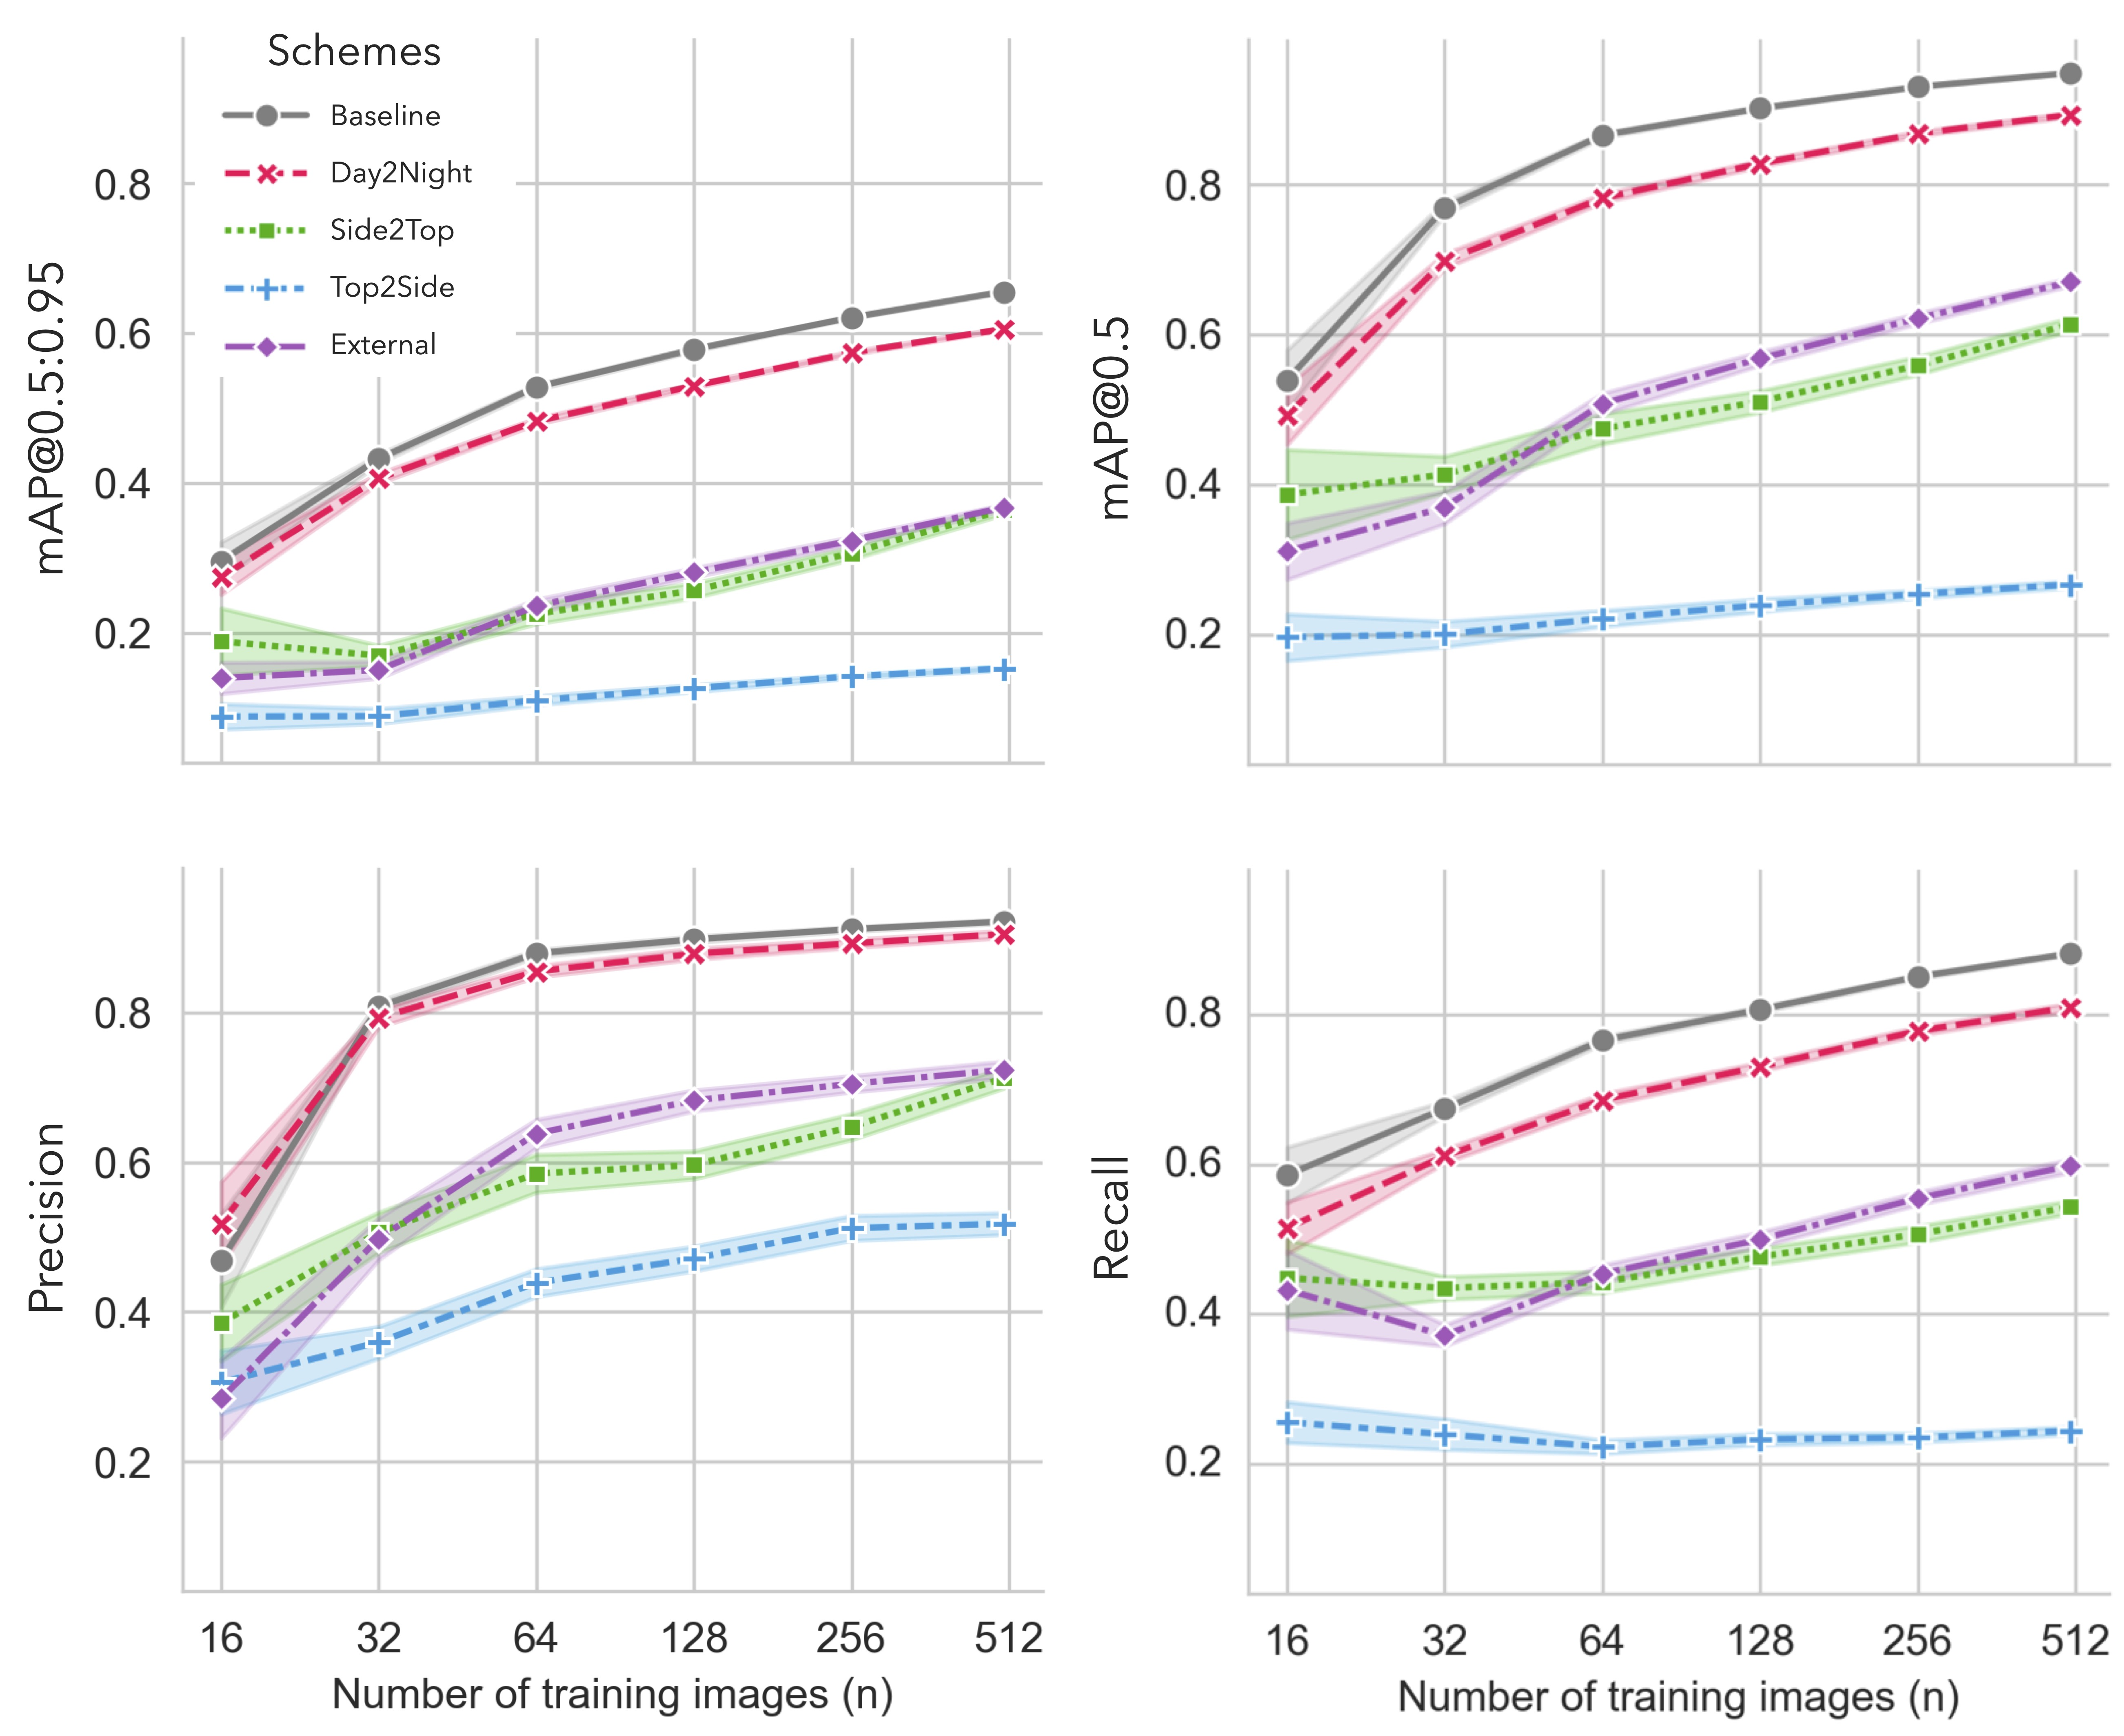
\includegraphics[width=0.8\textwidth]{figure_3.jpg}
    \caption{Examples of the annotated images.}
    \label{fig:schemes}
\end{figure}

The baseline training configuation show a good generalization capabiltiy, in which over 90\% of the predctions were correct in positioning cows at the criteria of 50\% IoU ($\text{mAP@{0.5}}$). Further, the generalization performance can be dissected into changes in view angles (i.e., Top2Side and Side2Top) and lighting condition (i.e., Day2Night). The lightinig condition changes did not dramatically affect the model performance in all four metrics, while changing camera views drop the performance by approxmiately 30\% and 60\% in ($\text{mAP@{0.5}}$ in the configurations of Side2Top and Top2Side, respectively. Across all the metrics and training sample sizes, the configuration of Top2Side consistently showed the worst performance. From the perspective of precision and recall, changing camera from top view to side view result in the model missing detecting more than 7 cows for ever 10 cows and only 50\% of the detection were correct. It is noted that the performance in the Day2Night configuration is closed to the baseline in the metric precision, which only consider predictions with high confidence compared to the metric ($\text{mAP@{0.5}}$). Hence, by excluding the low-confidence predictions, changing ligthing condition did not affect the model performance. Regardless of the configuration and the evaluation metrics, the model performances always increase as the trianing sampel sizes increase.


\subsection*{Study 2: A higher model complexity does not always lead to better performance}


\begin{figure}[h]
    \centering
    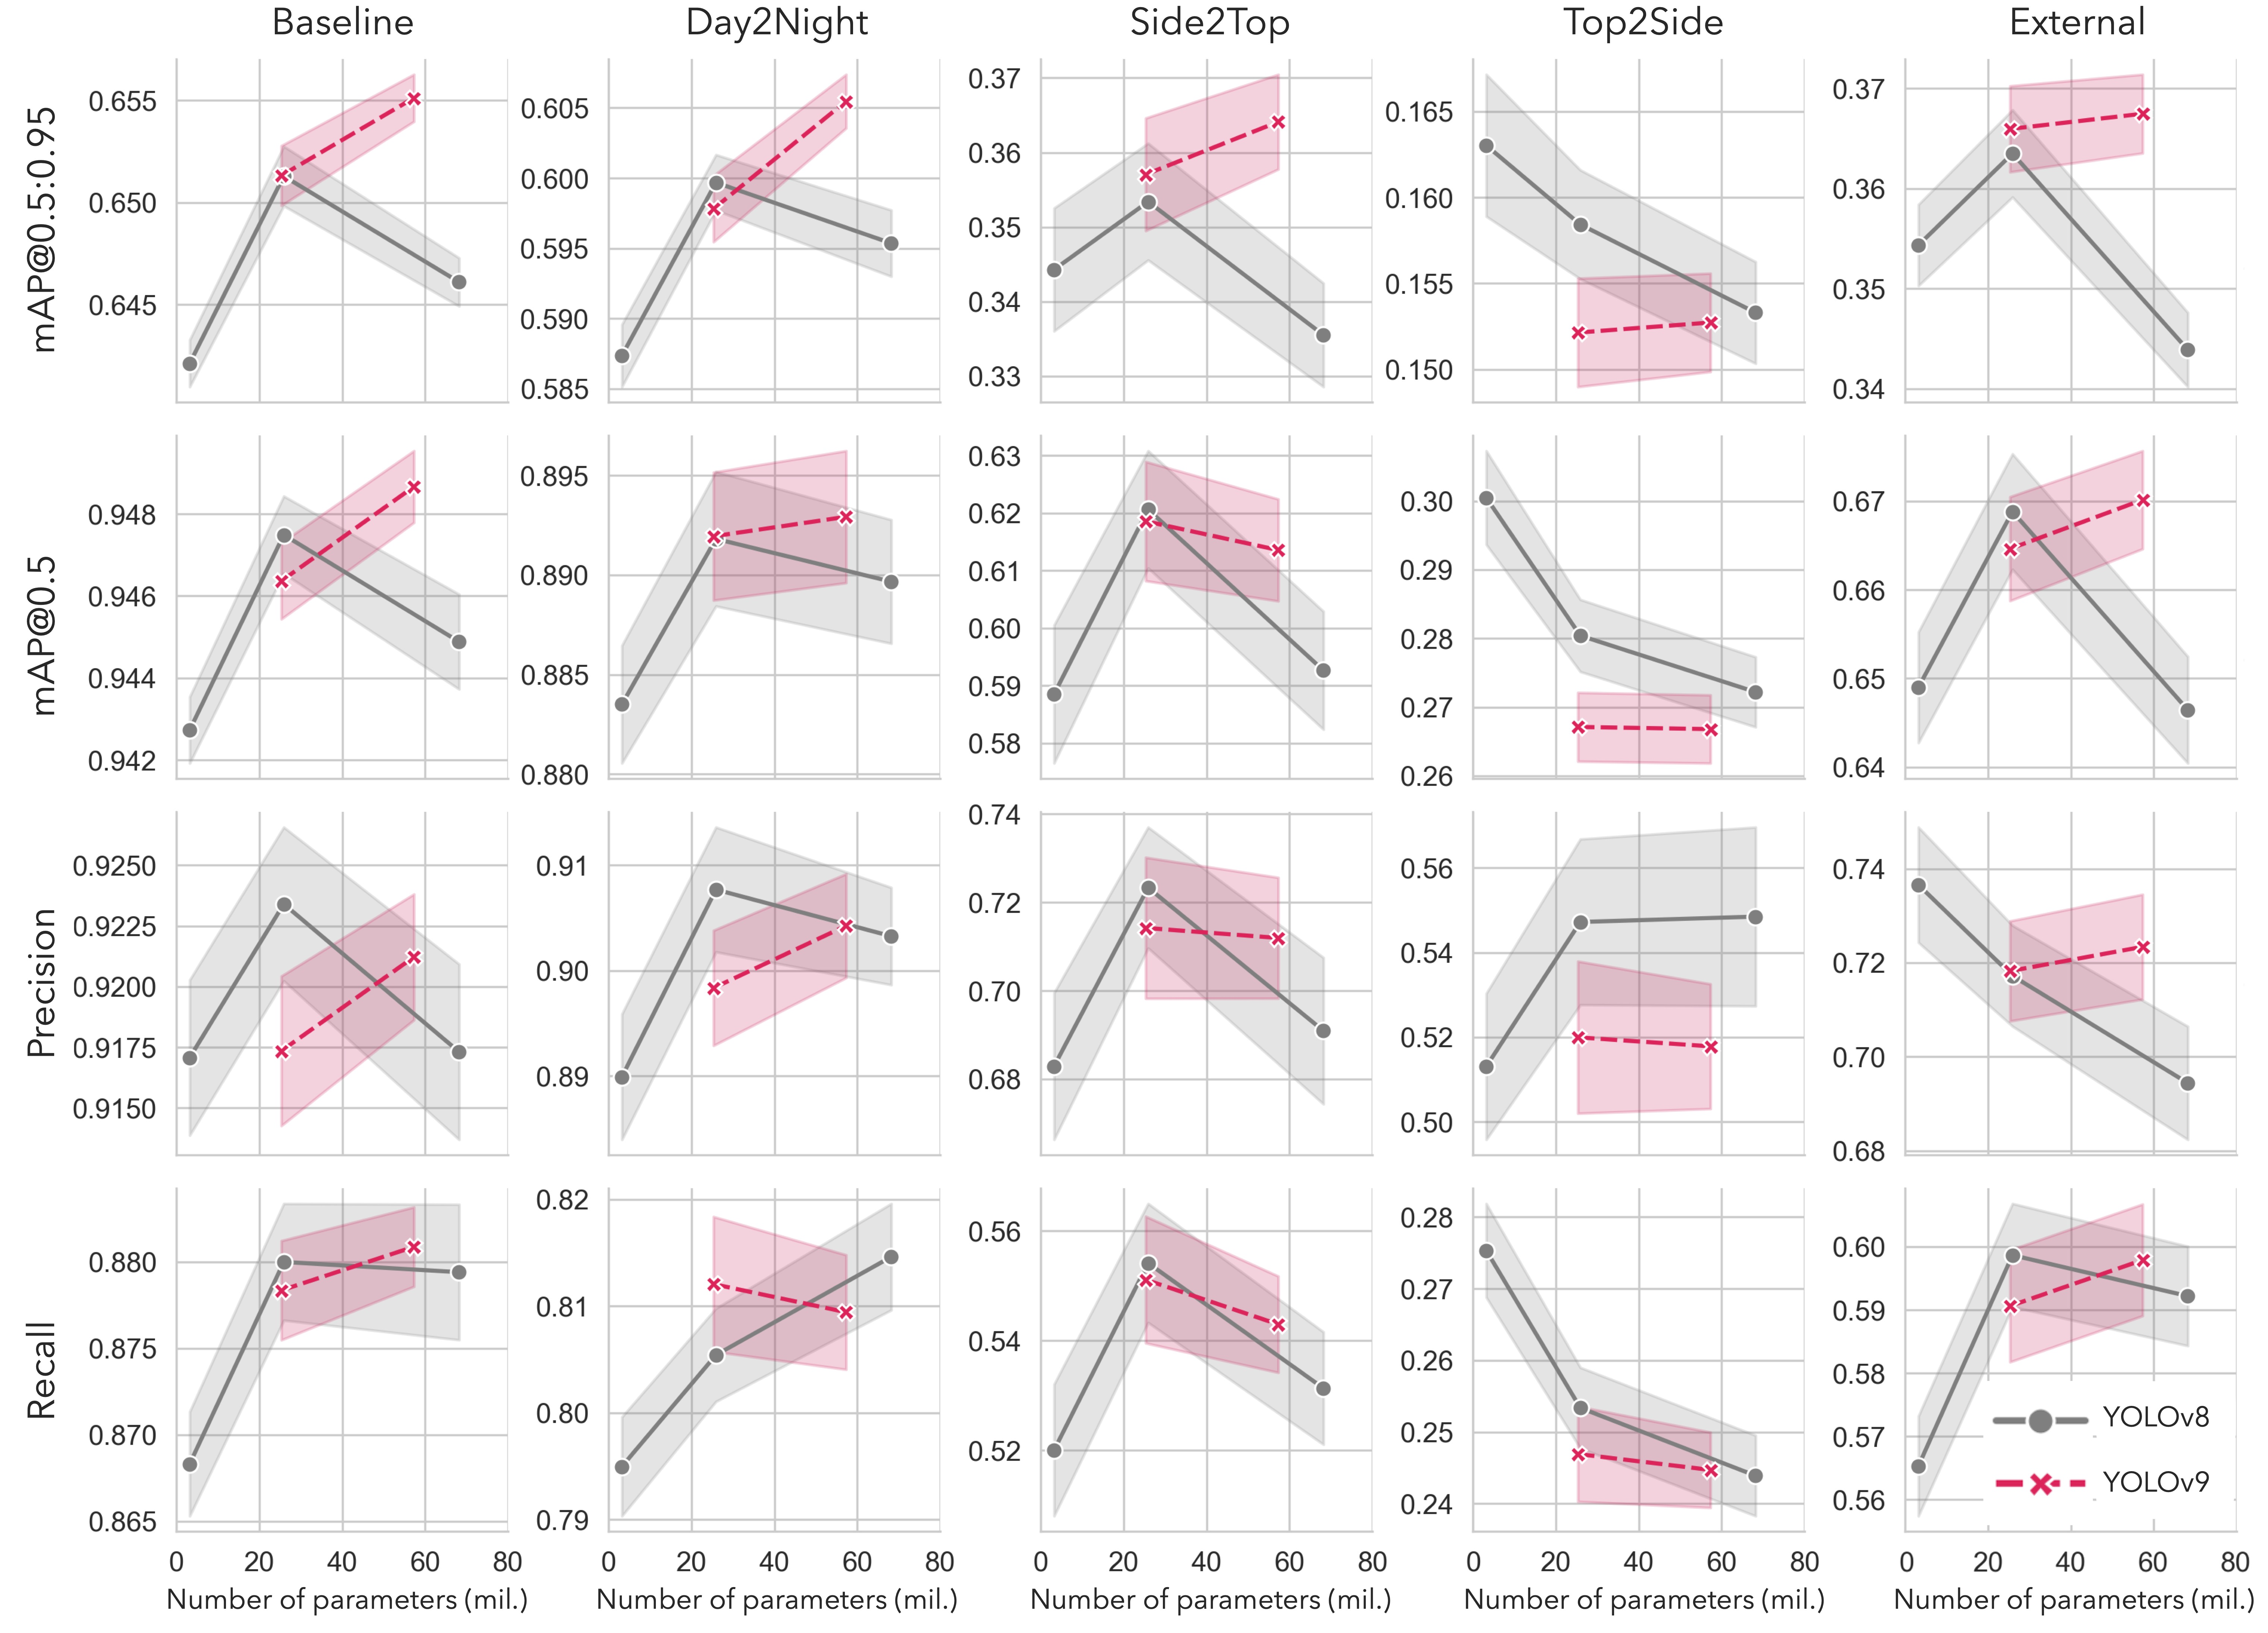
\includegraphics[width=1\textwidth]{figure_4.jpg}
    \caption{Examples of the annotated images.}
    \label{fig:models}
\end{figure}


From the study, it is found that the xxx of the training configuration affects the relationship between the model complexity and the performance. Based on the study 1, predicting images from the side view based on the model trained on from the top-view camera is the most challenging tasks. In this configuration, increasing the model complexity, except for few cases, the model generalization always became worse than the simple models are. However, in other configurations that show better generalization in the Study 1, the peak performance did not always found from the most complex model. For example, in the baseline, the model that performed that best is YOLOv9e in metrics of $\text{mAP@{0.5:0.95}}$, $\text{mAP@{0.5}}$, and recall. And YOLOv8m performed the best in precision. Neither of the model has the most parameter counts compared to YOLOv8x. It is also worth noting that, different model architecture show different trend in the performance over model complexity. The YOLOv8-family models more likely to have the best performance with the mid-sized model (i.e., YOLOv8m). While in YOLOv9, larger models usually performed better. Hence, the study concluded that the model performacne is determined by both training configuration and the model archtecture.


\begin{figure}[h]
    \centering
    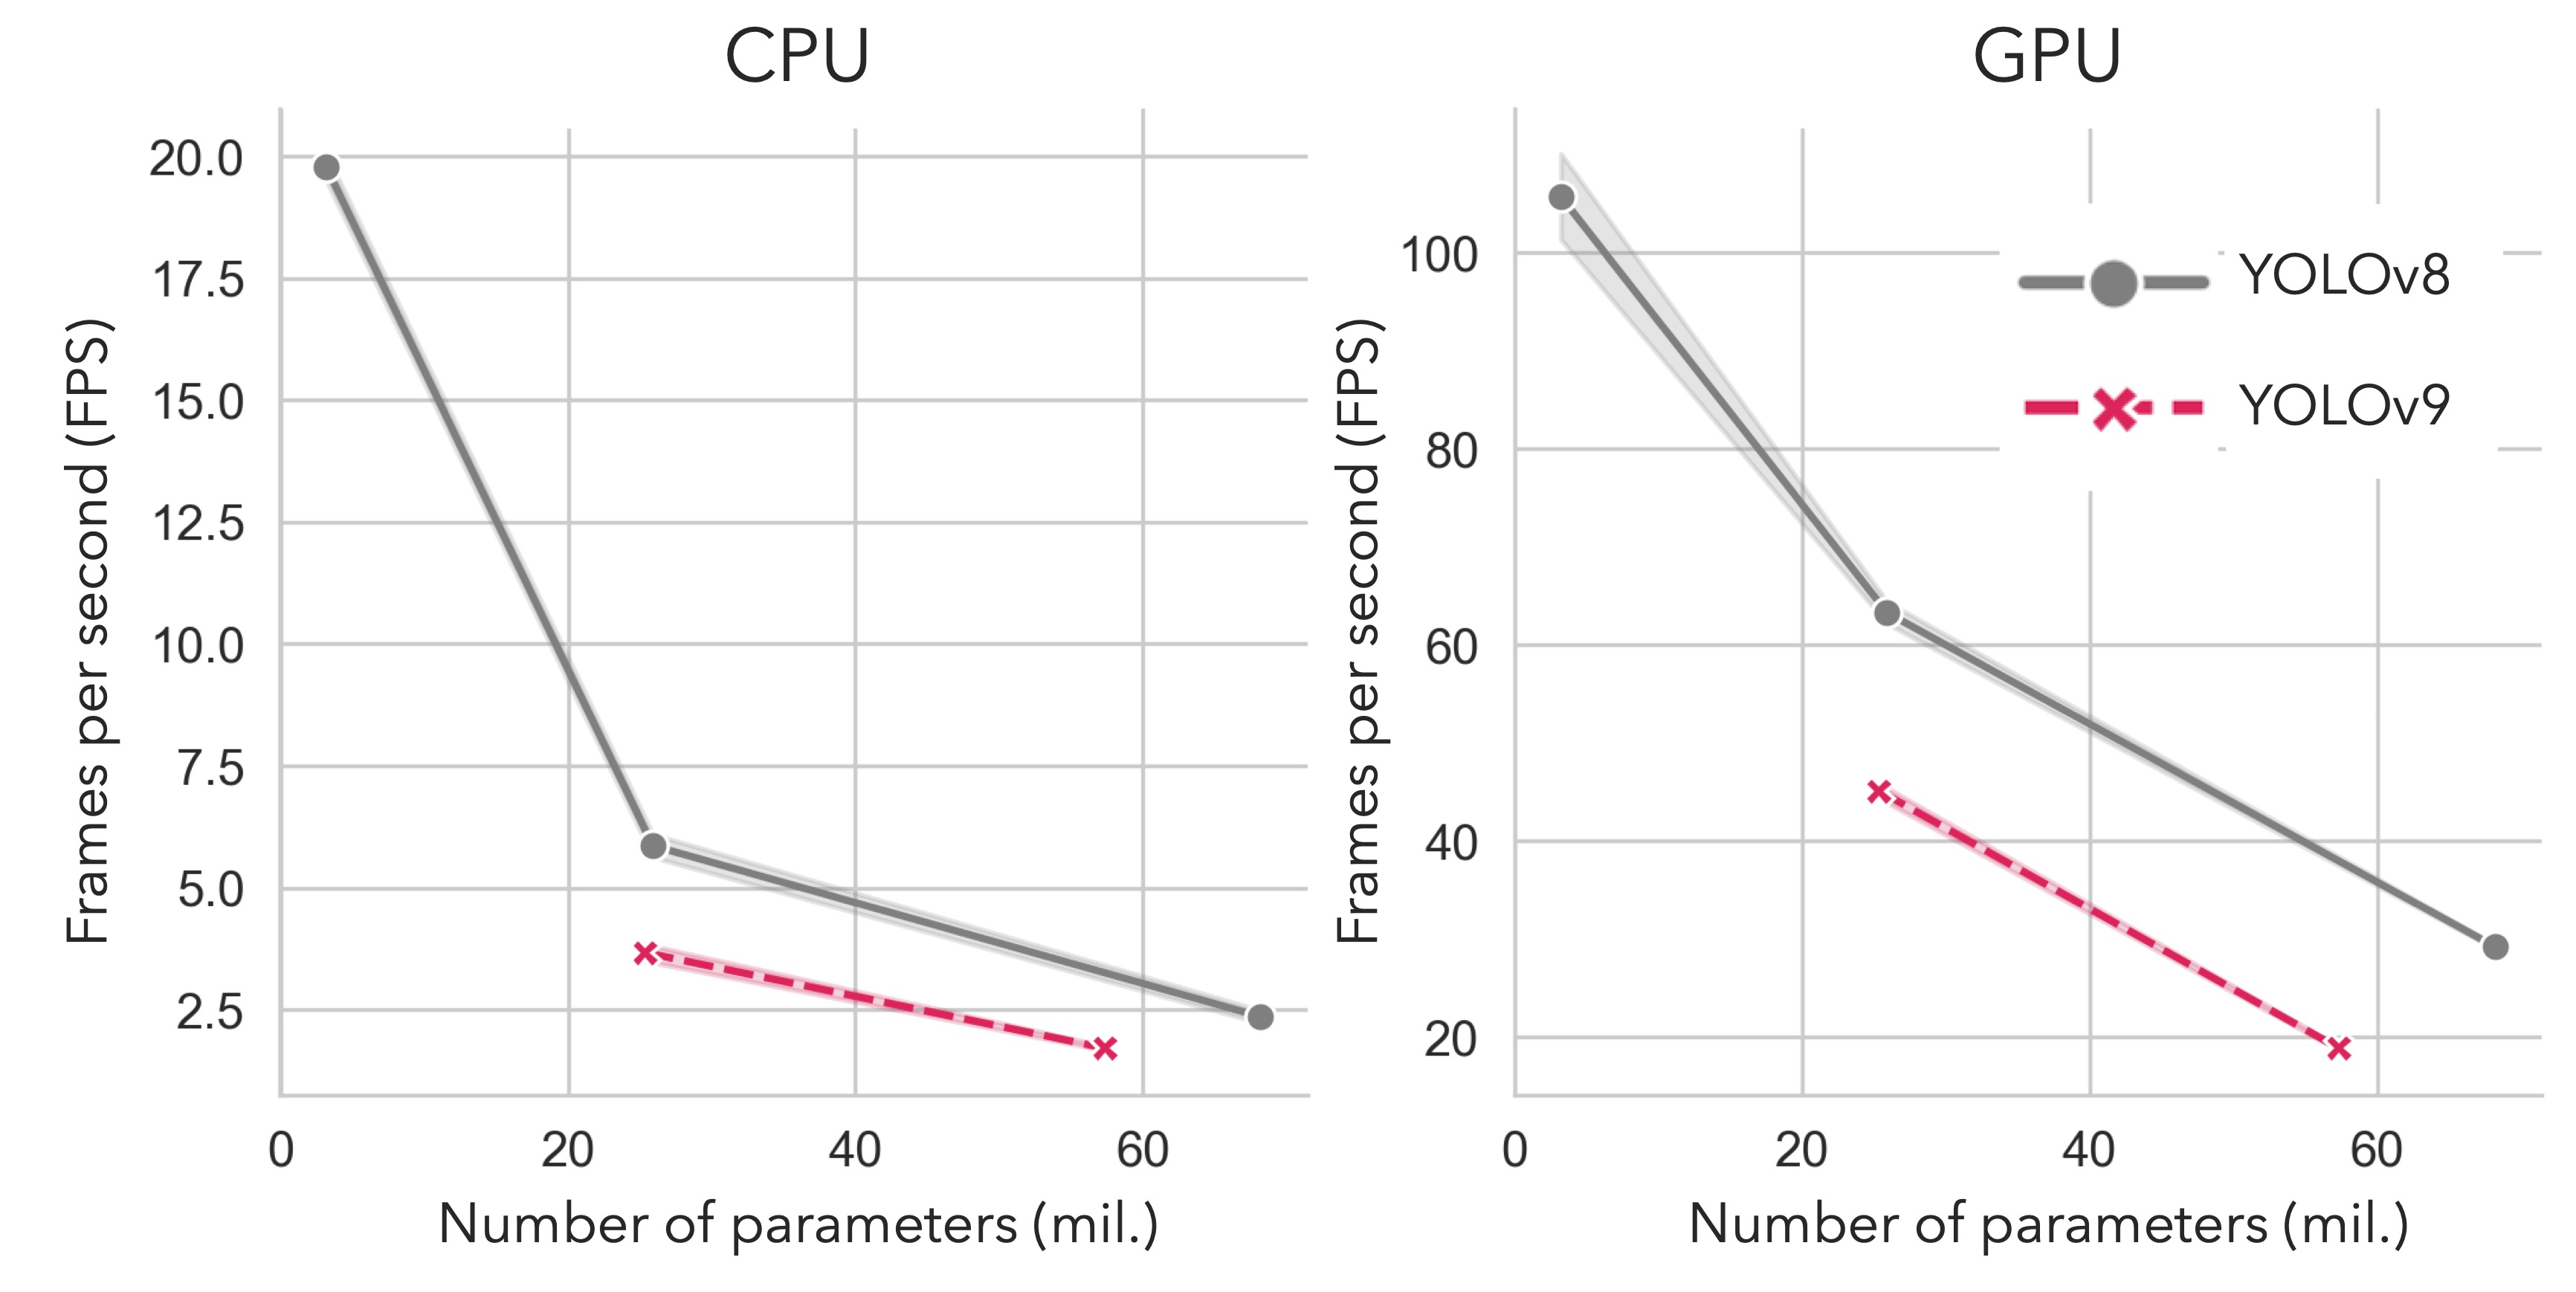
\includegraphics[width=.6\textwidth]{figure_6.jpg}
    \caption{Examples of the annotated images.}
    \label{fig:inference}
\end{figure}


\subsection*{Study 3: The advantages started to disminish early as the training sample sizes when the model is simple}



\begin{figure}[h]
    \centering
    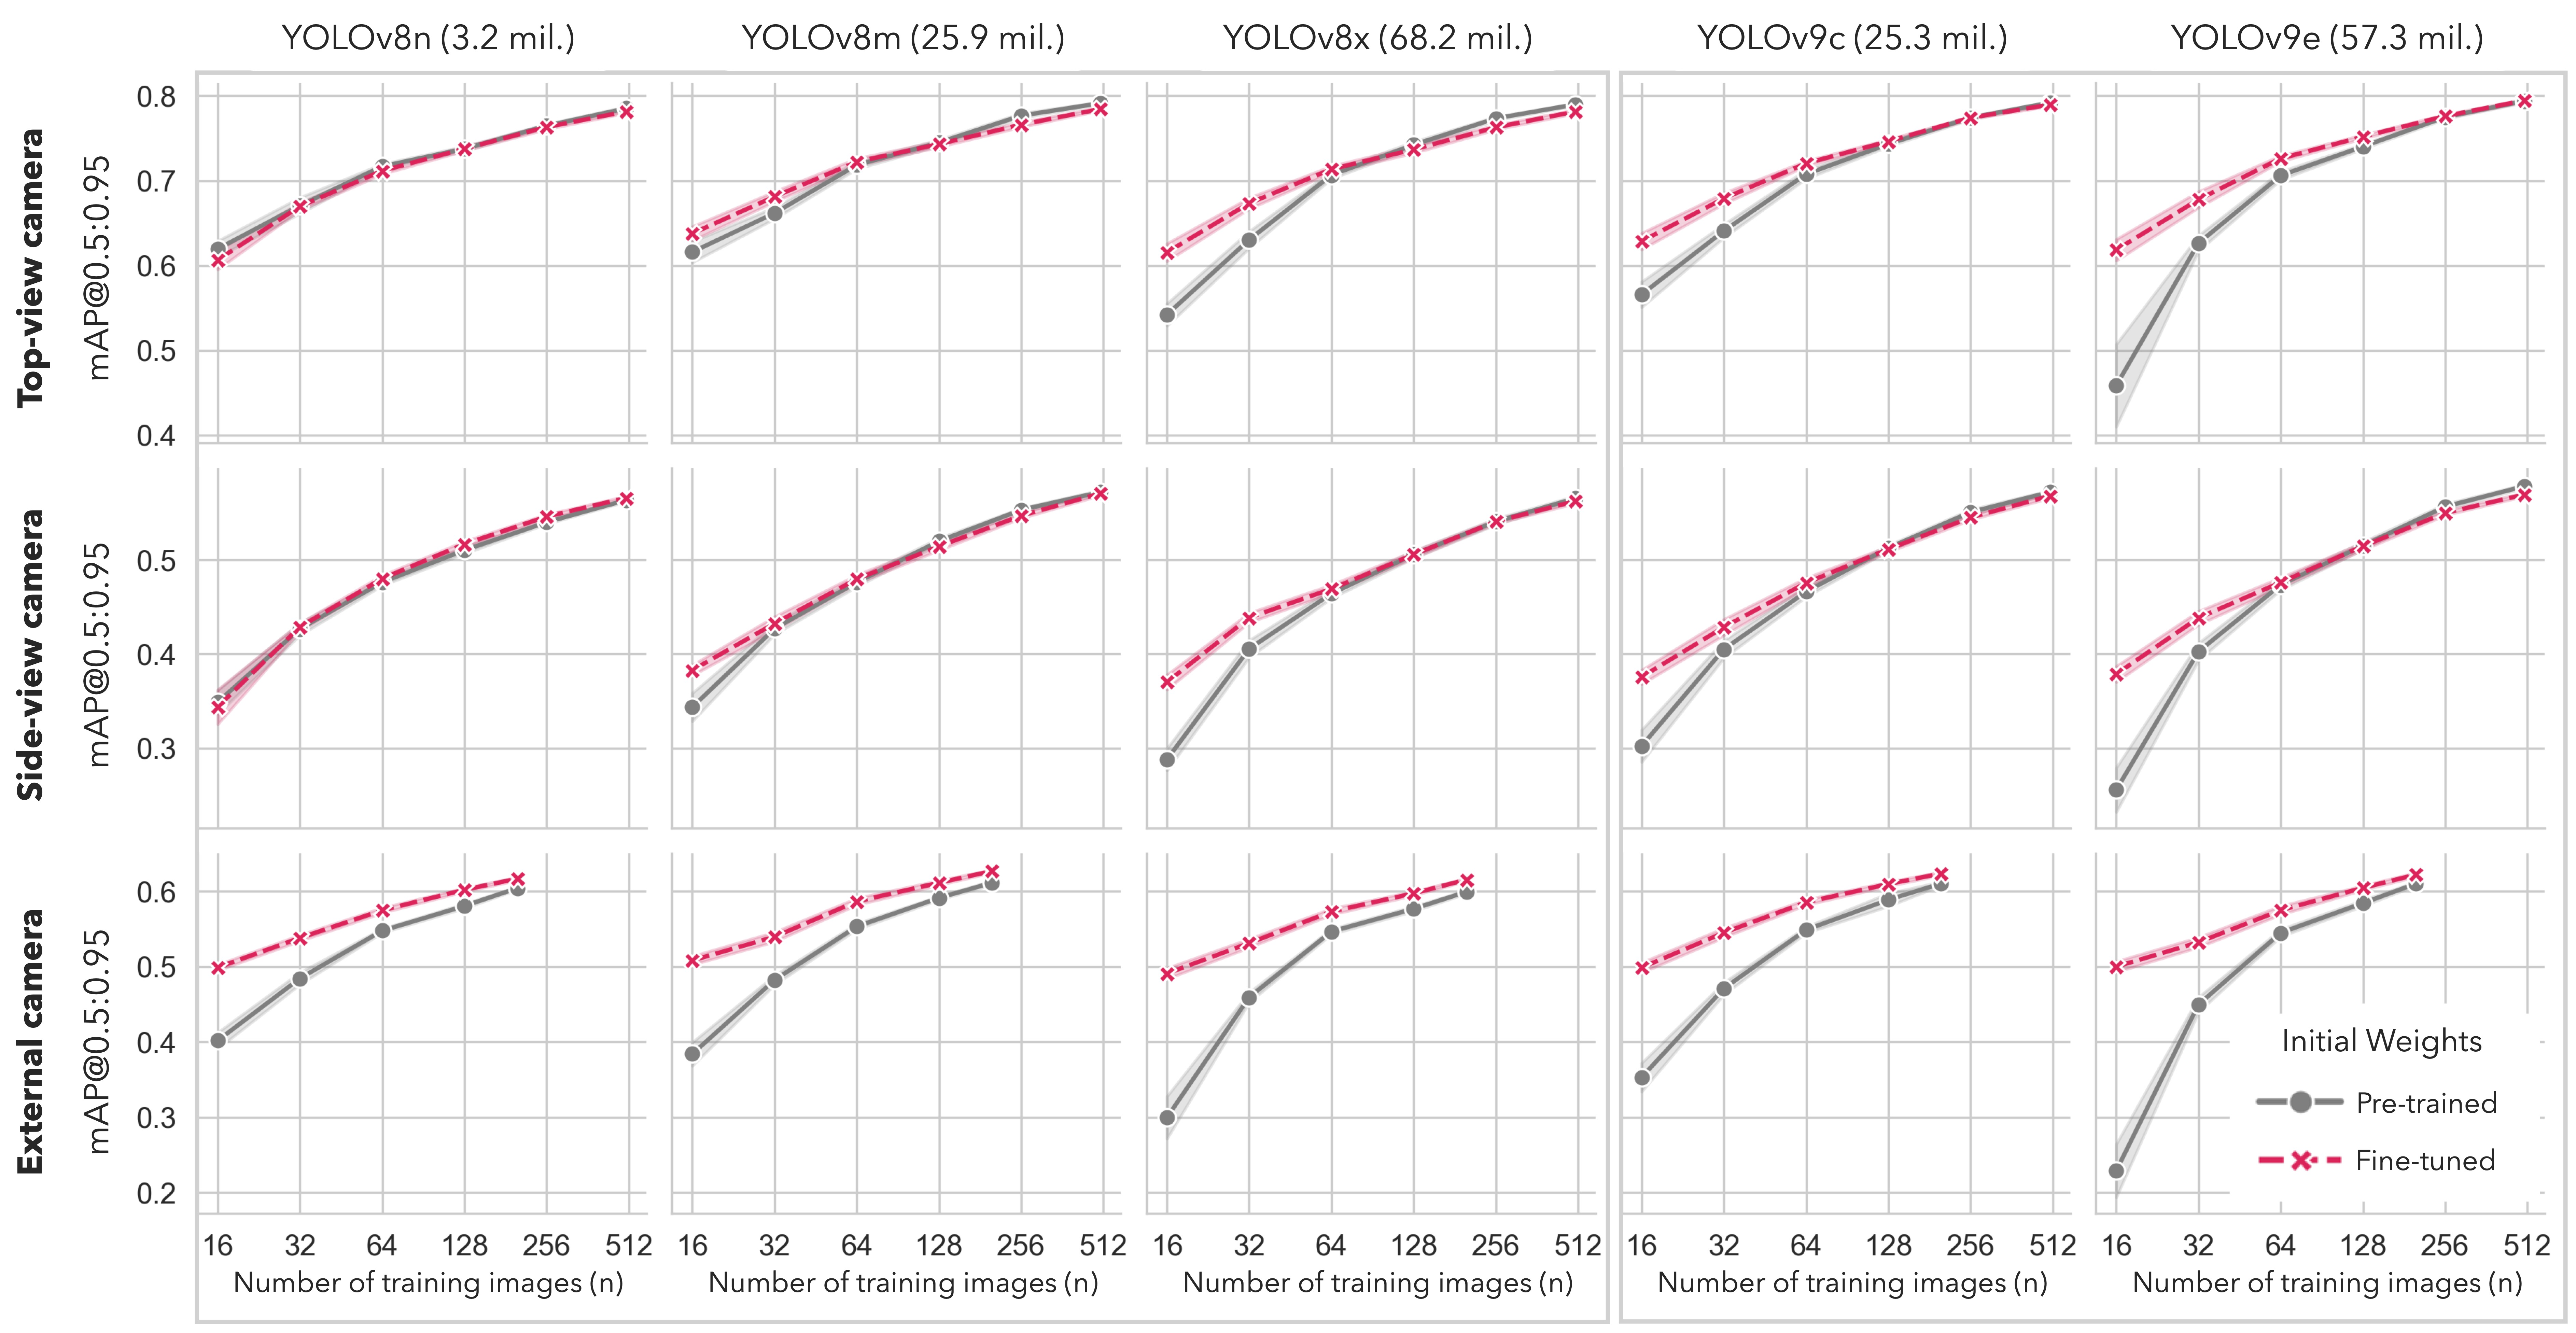
\includegraphics[width=1\textwidth]{figure_5.jpg}
    \caption{Examples of the annotated images.}
    \label{fig:finetune}
\end{figure}

